\subsection{MQuicTT binary composition} \label{sec:binary_sizes}

We first look at an in-depth breakdown of the MQuicTT binary and analyse the contribution to the QUIC stack.
Figure~\ref{fig:mquictt_client_bin} shows the result of the binary breakdown by crate.

\begin{figure}[ht]
    \centering
    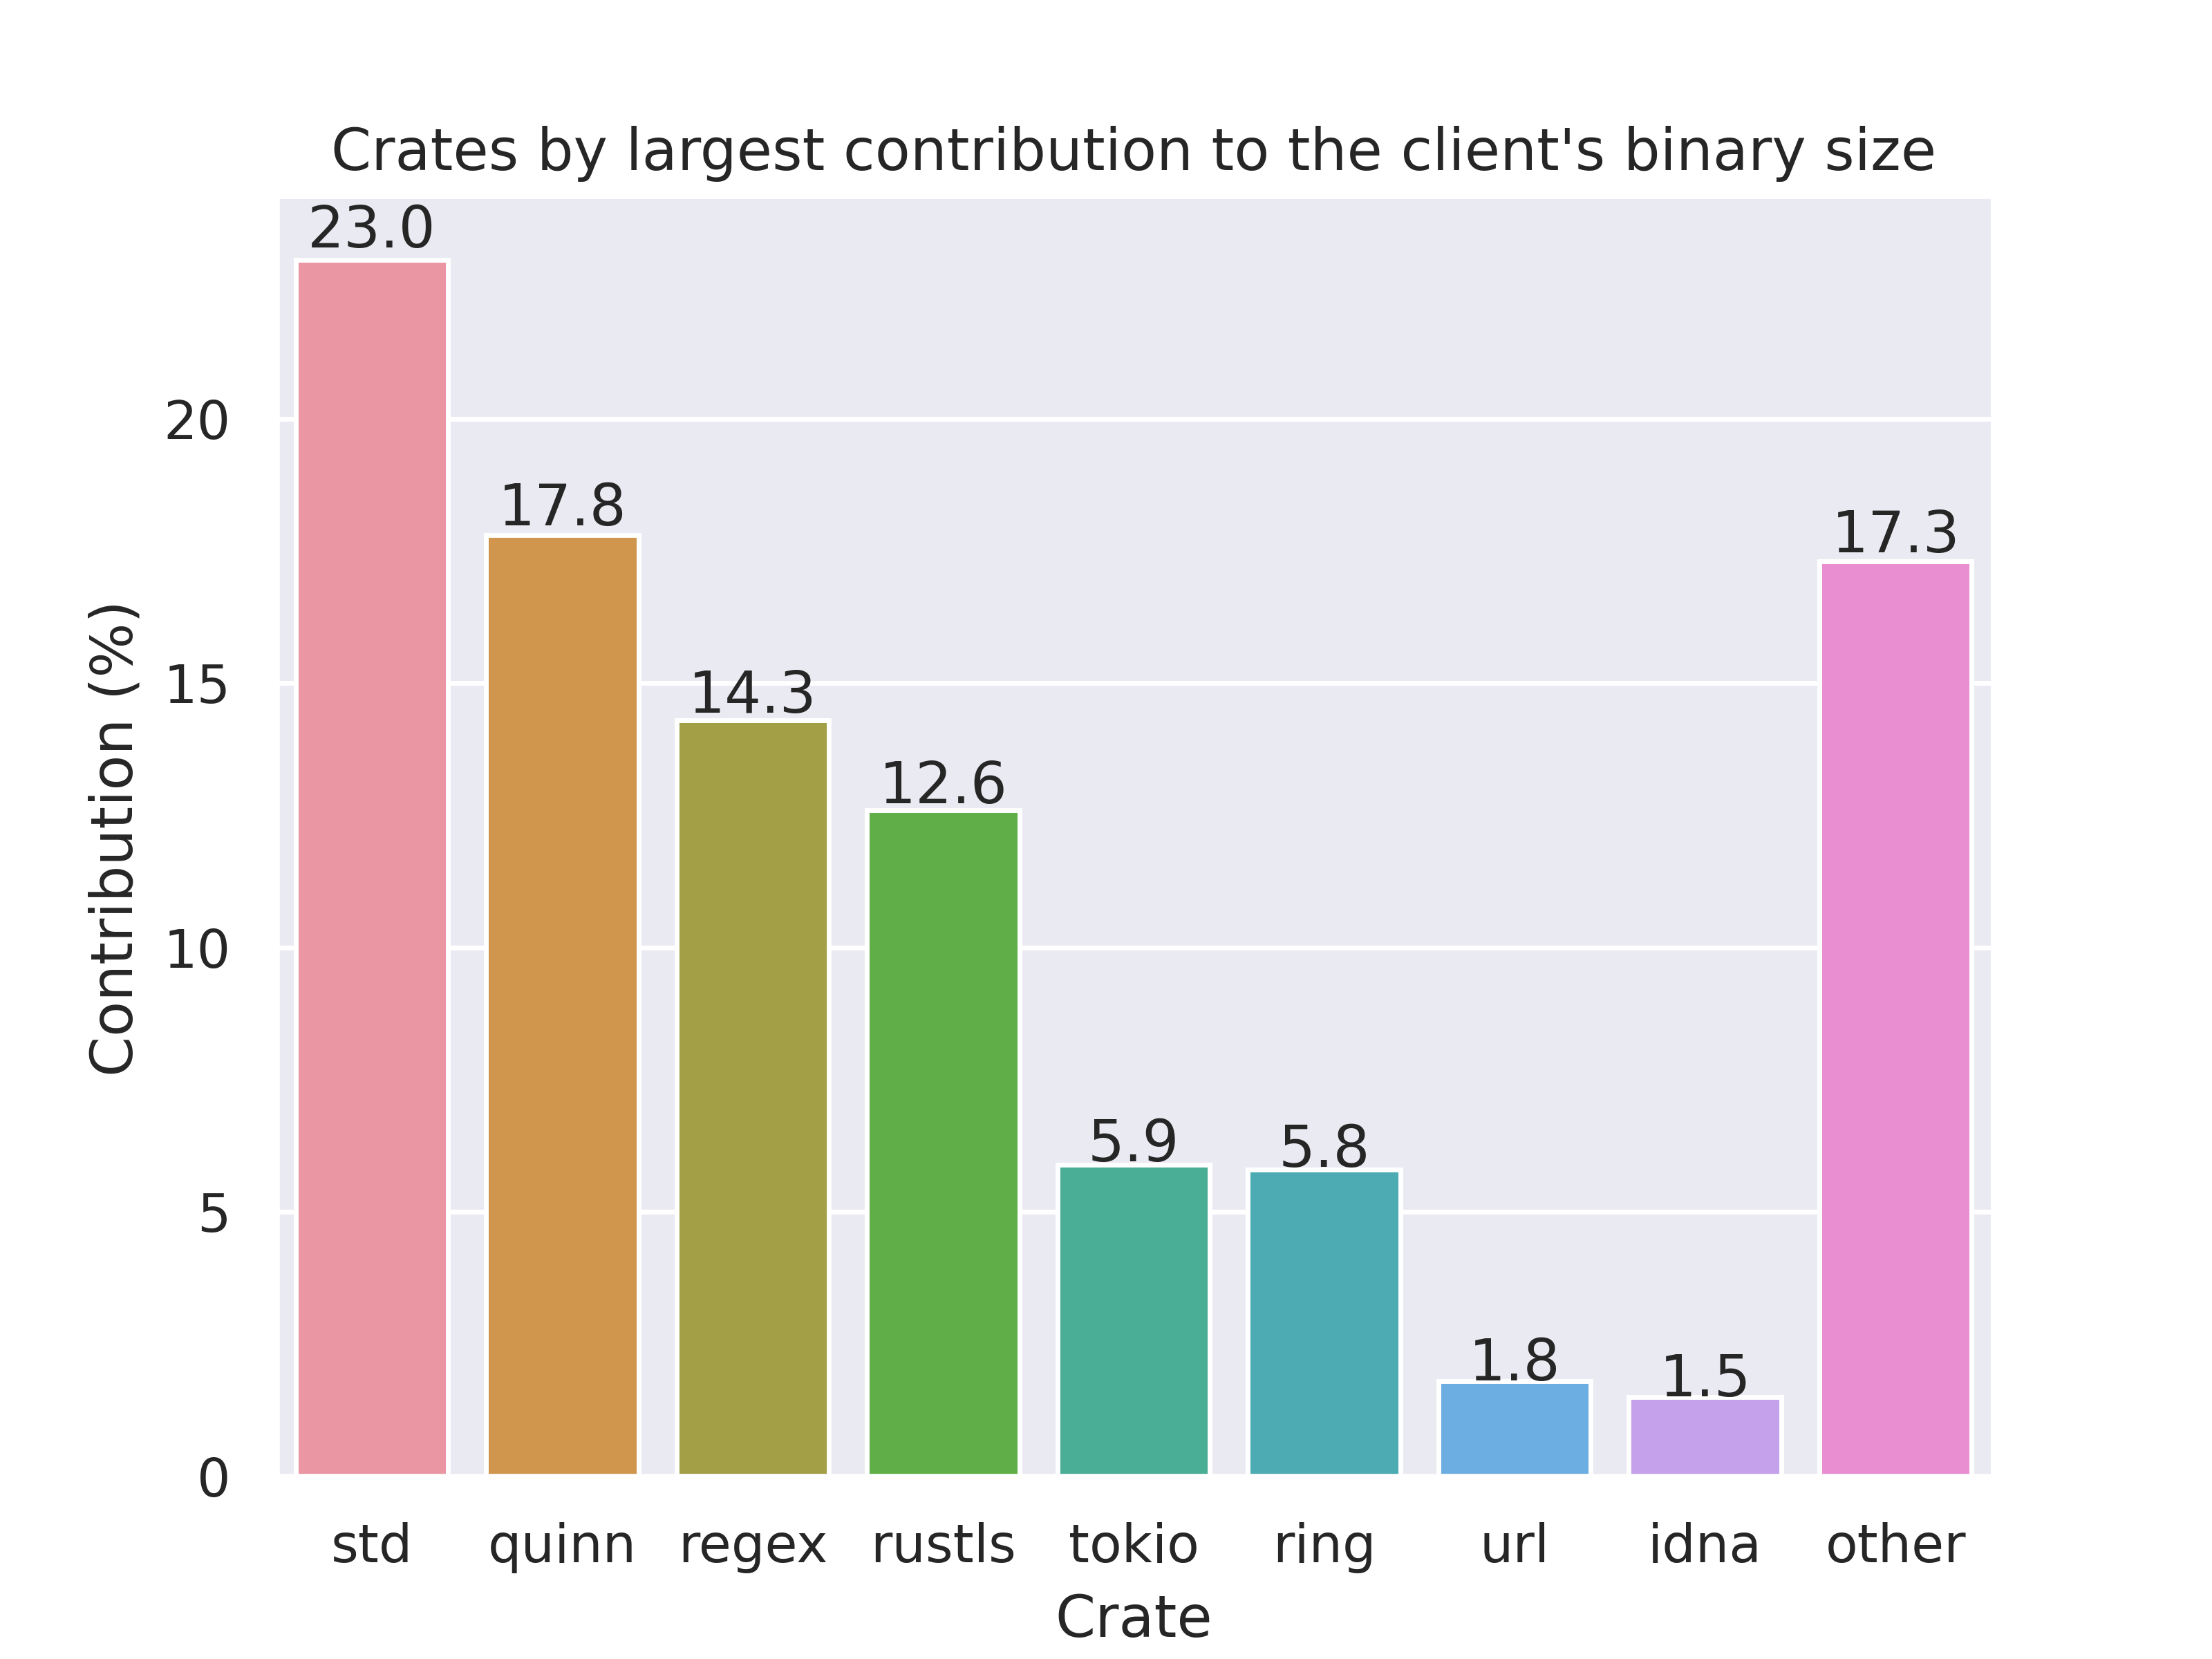
\includegraphics[width=1\linewidth]{images/mquictt_binary_client.png}
    \caption{Top contributions to the binary size of the MQuicTT client by crate. That is, which libraries contribute the largest footprint.}
    \label{fig:mquictt_client_bin}
\end{figure}

When analysing the QUIC stack contribution to the binary size, we can see that $quinn$ contributes to $17.8\%$ of the binary size and $rustls$ contributes a further $12.6\%$.
Additionally, we can see that the $ring$ crate contributes another $5.8\%$.
This crate is a Rust binding for BoringSSL primitives; hence it is part of the TLS implementation.
Overall, this means that the QUIC stack constitutes $36.2\%$ of MQuicTT's client binary size.
This result is in line with our prediction that the QUIC stack will contribute the most to the binary size.

Unexpectedly, however, the $regex$ crate contributes $14.3\%$ to the size of the client binary exceeding even the contribution made by the TLS implementation.
This can partially be attributed to Rust's support for Unicode in strings.
Specifically, a $char$ type in Rust represents a Unicode scalar value, a Unicode version agnostic type.
While providing many wanted features, Rust's native support for Unicode also increases the used resources.
A possible workaround would be to add optional support for the $unicase::Ascii$ type to the $regex$ crate.
Another possible reason for the size of this crate is the source codes extensive use of the $inline(always)$ annotation.
This annotation tells the compiler to inline functions across crate boundaries, possibly contributing to the binary size.
Overall, we can see that this anomaly can be attributed to the choice of programming language, which presents an insight into Rust as a language for hardware constrained devices.

We can also see that despite other crates not contributing a considerable amount towards the binary size, cumulatively, their size adds up to $17.3\%$ of the binary size due to the large number of them.
We have found over 40 crates that contributed to this, including data structure implementations, lower-level network interfaces, abstractions on byte buffers and logging utilities.
Notably, we have found that logging utilities and error reporting do not largely contribute to the size of the client's binary.
This comes in contrast to one of the steps in reducing the binary size taken by~\cite{eggert_towards_2020}.

Figure~\ref{fig:mquictt_broker_bin} shows similar results for MQuicTT's broker.
We can see that in the case of the broker, the QUIC stack constitutes $32.9\%$ of the binary size.
Similarly to the client, the $regex$ crate again shows a large binary size footprint, and the lesser crates contribute to a sizeable cumulative amount.
Additionally, similarly to the results presented for the client, we have found that the logging and error checking crates have not contributed largely to the binary size.

\begin{figure}[ht]
    \centering
    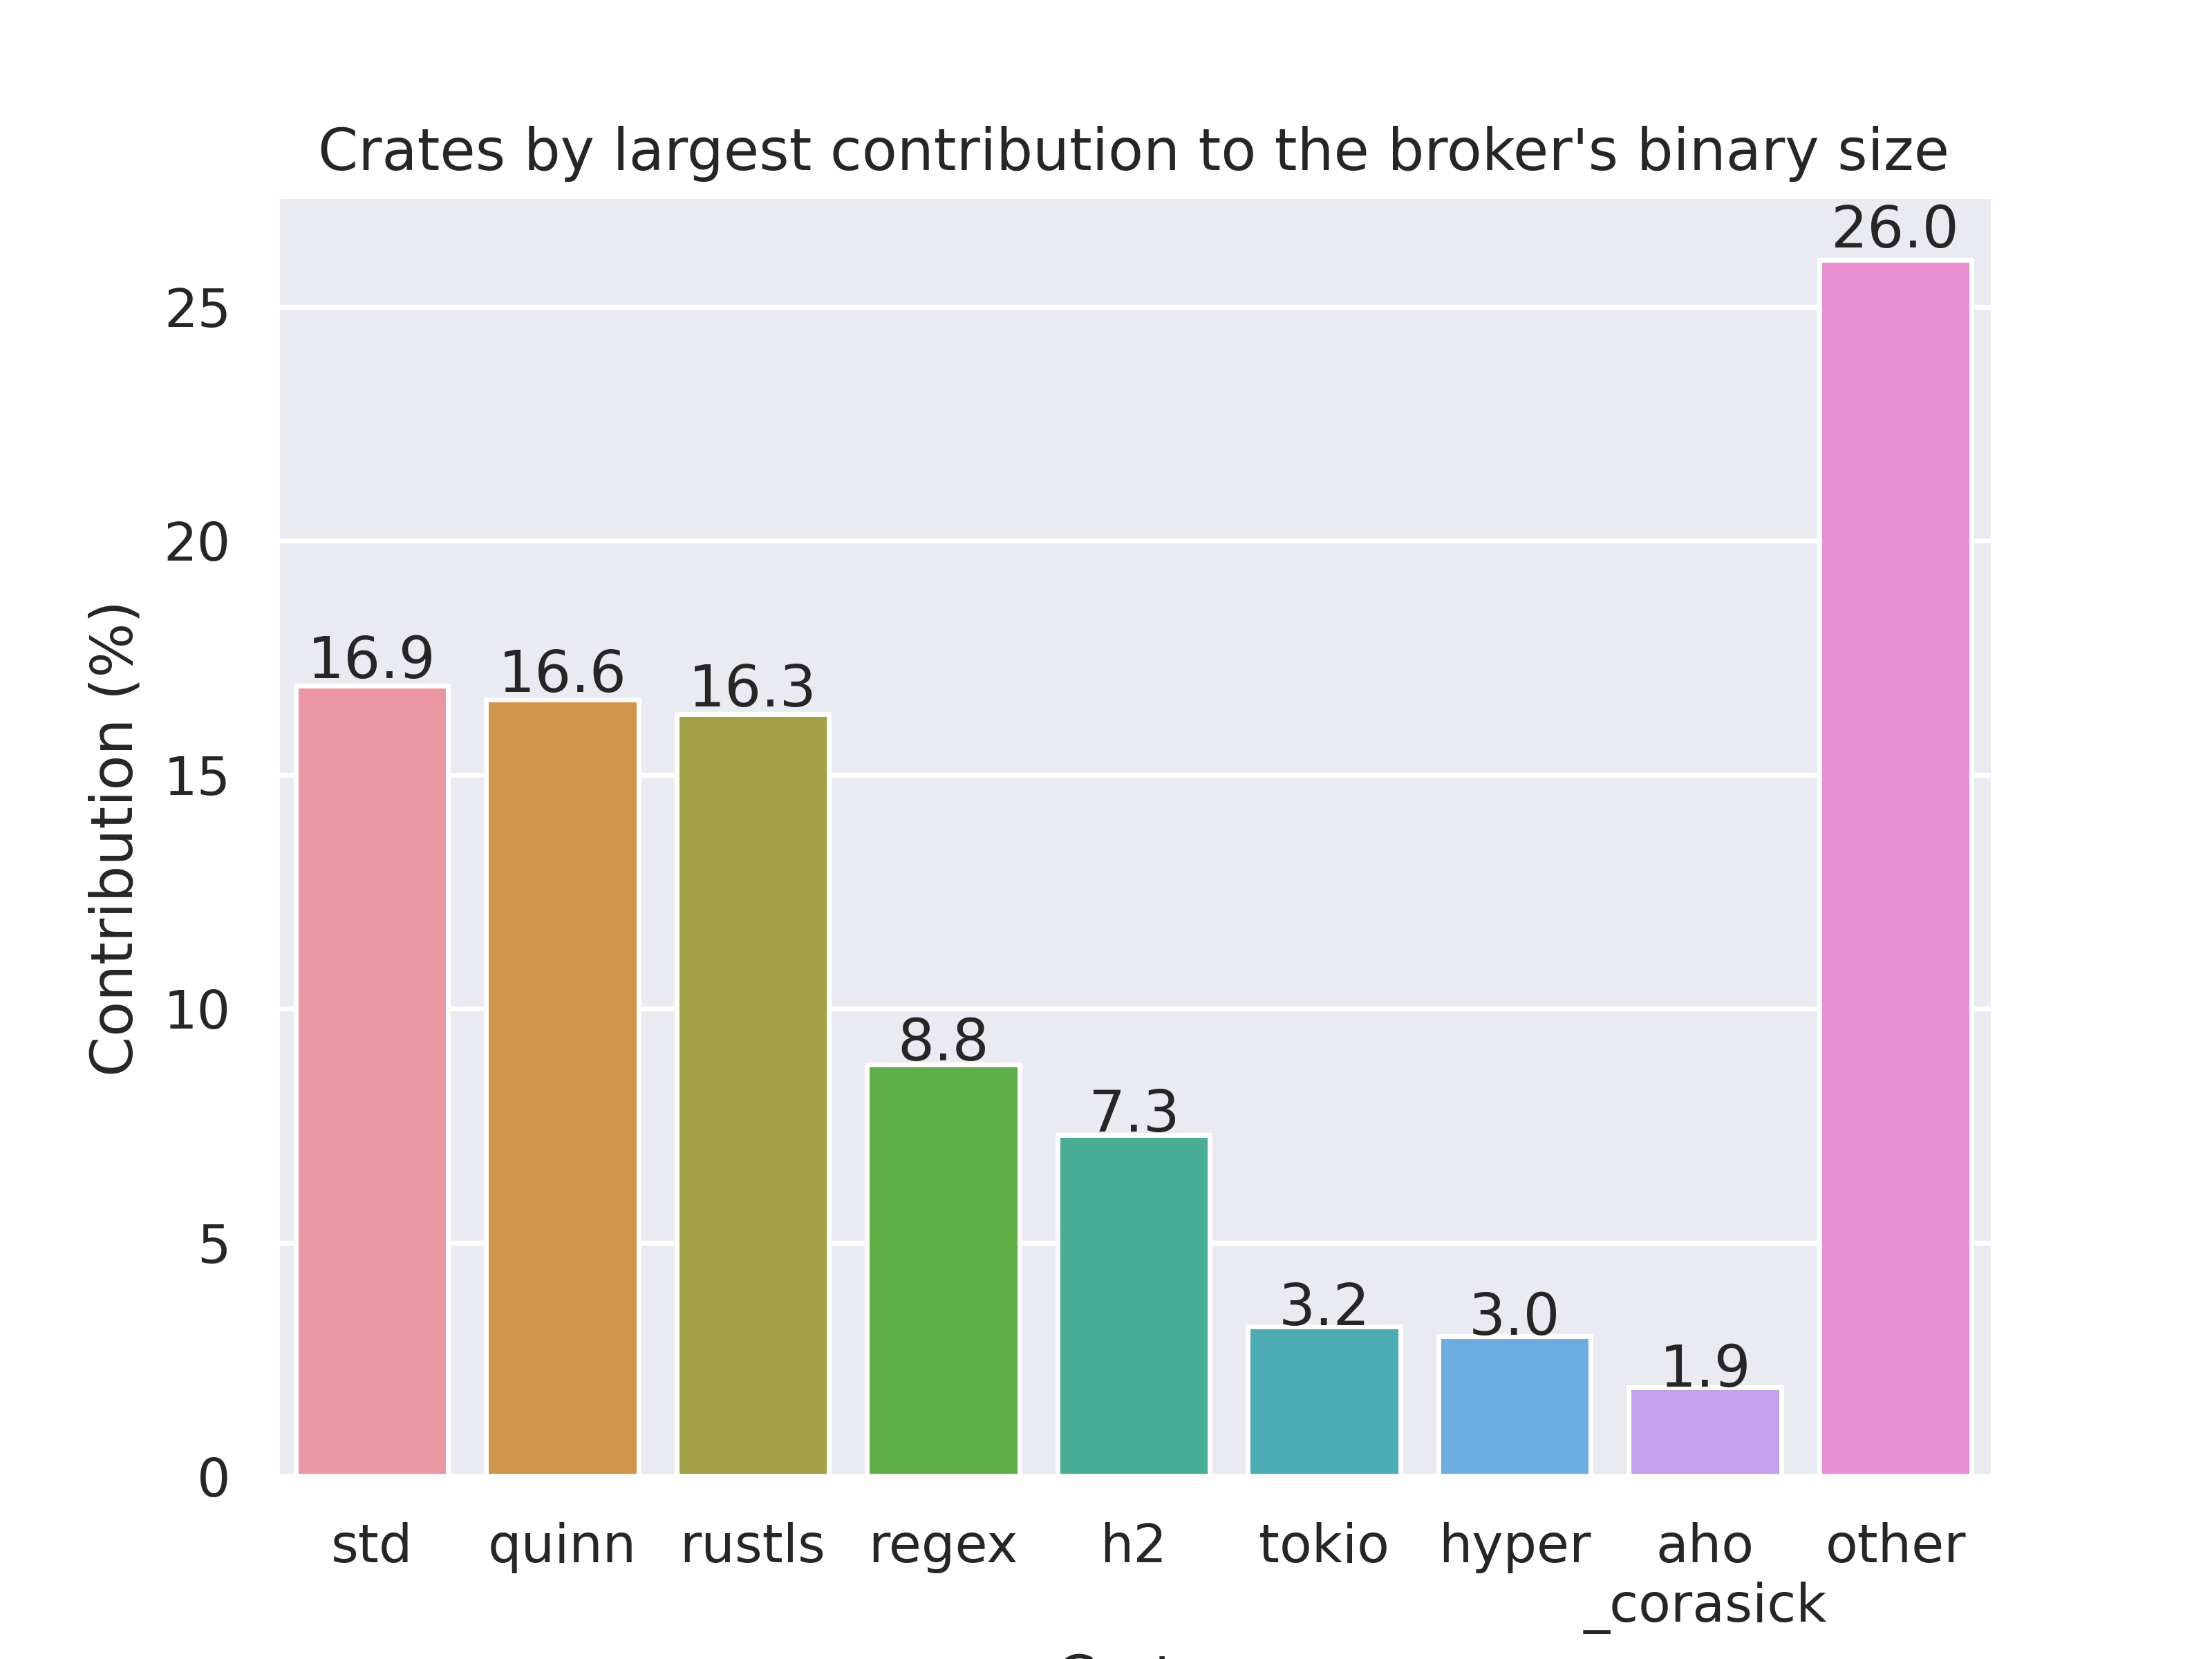
\includegraphics[width=1\linewidth]{images/mquictt_binary_broker.png}
    \caption{Top contributions to the binary size of the MQuicTT broker by crate. That is, which libraries contribute the largest footprint.}
    \label{fig:mquictt_broker_bin}
\end{figure}

We have further analysed the binary to see which methods contribute to the size for the client and broker.
Notably, in both cases, the $quinn\_proto$ module of $quinn$ contains several methods such as $connection::Connection::process\_payload$ and $endpoint::Endpoint::handle$ that each contribute around $0.8\%$.
Notably, however, the $regex::exec::ExecBuilder::build$ method from the $regex$ crate contributes $0.7\%$, which is a larger contribution than $quinn's$ methods for decrypting packets and polling for connections.

\begin{figure}
    \begin{center}
        \begin{subfigure}[b]{1\textwidth}
            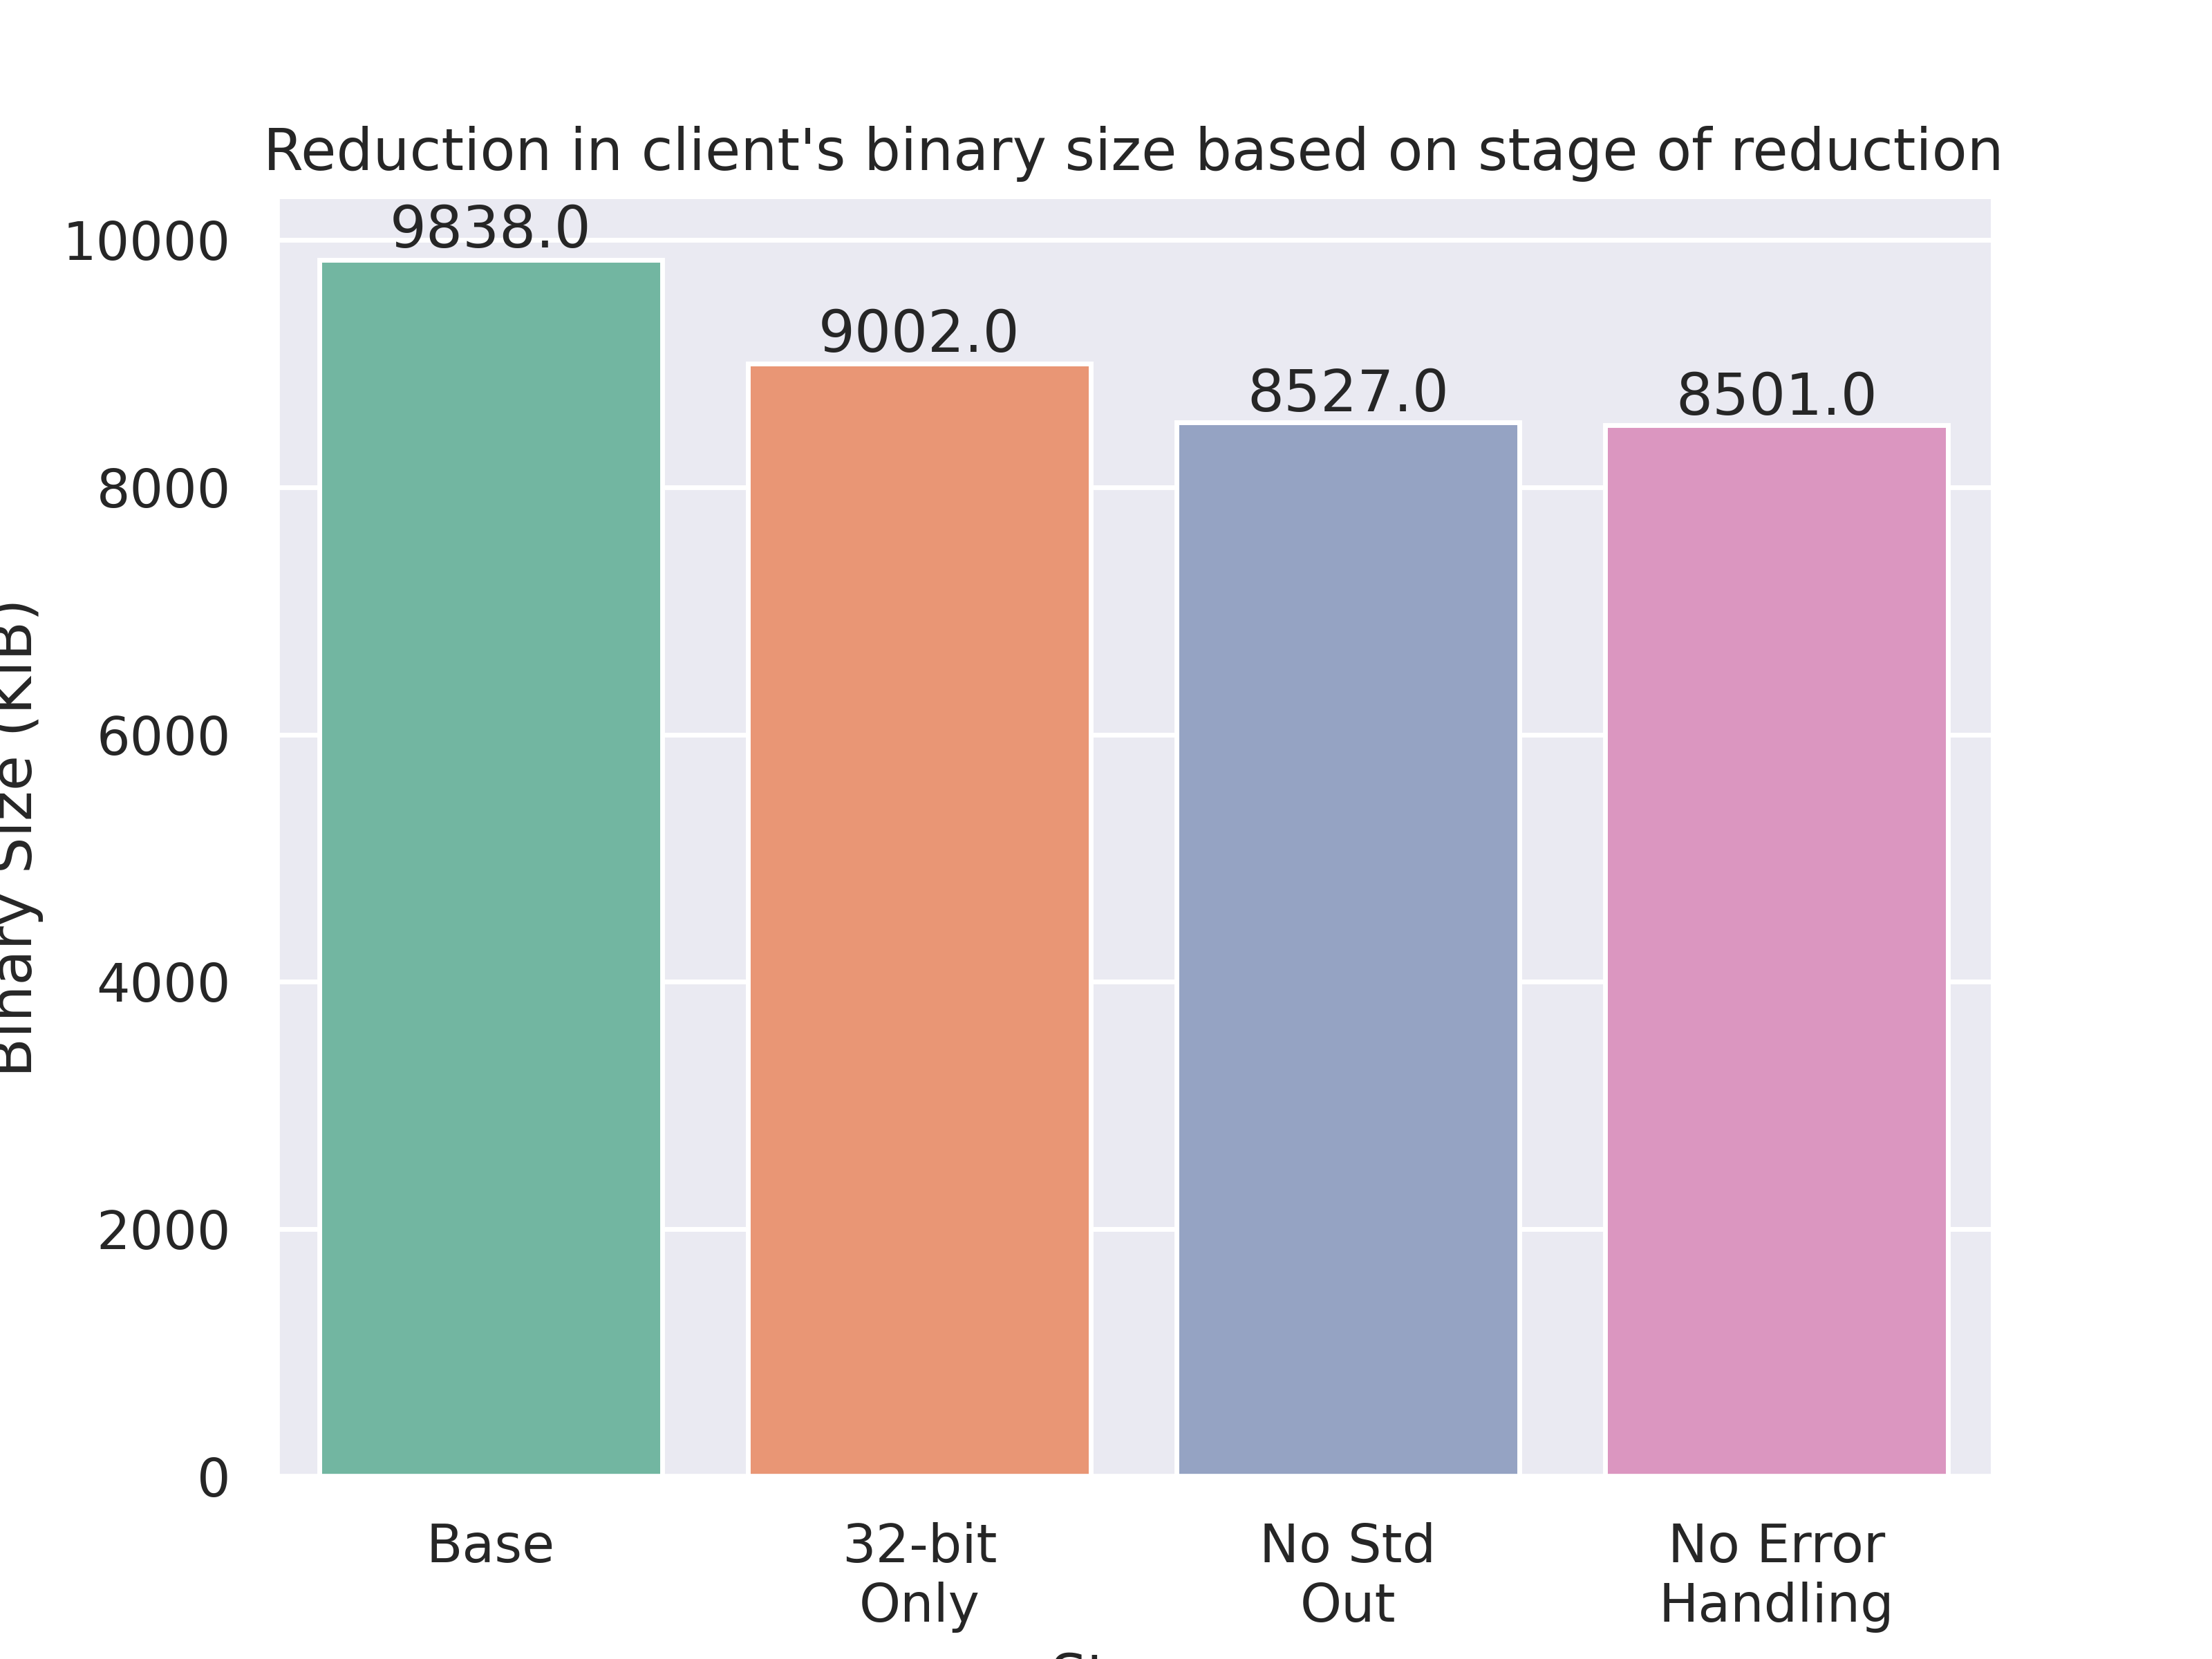
\includegraphics[width=1\linewidth]{images/quinn_binary_reduce_client.png}
            \caption{Client binary size reduction.}
            \label{fig:reduce_client}
        \end{subfigure}
        \begin{subfigure}[b]{1\textwidth}
            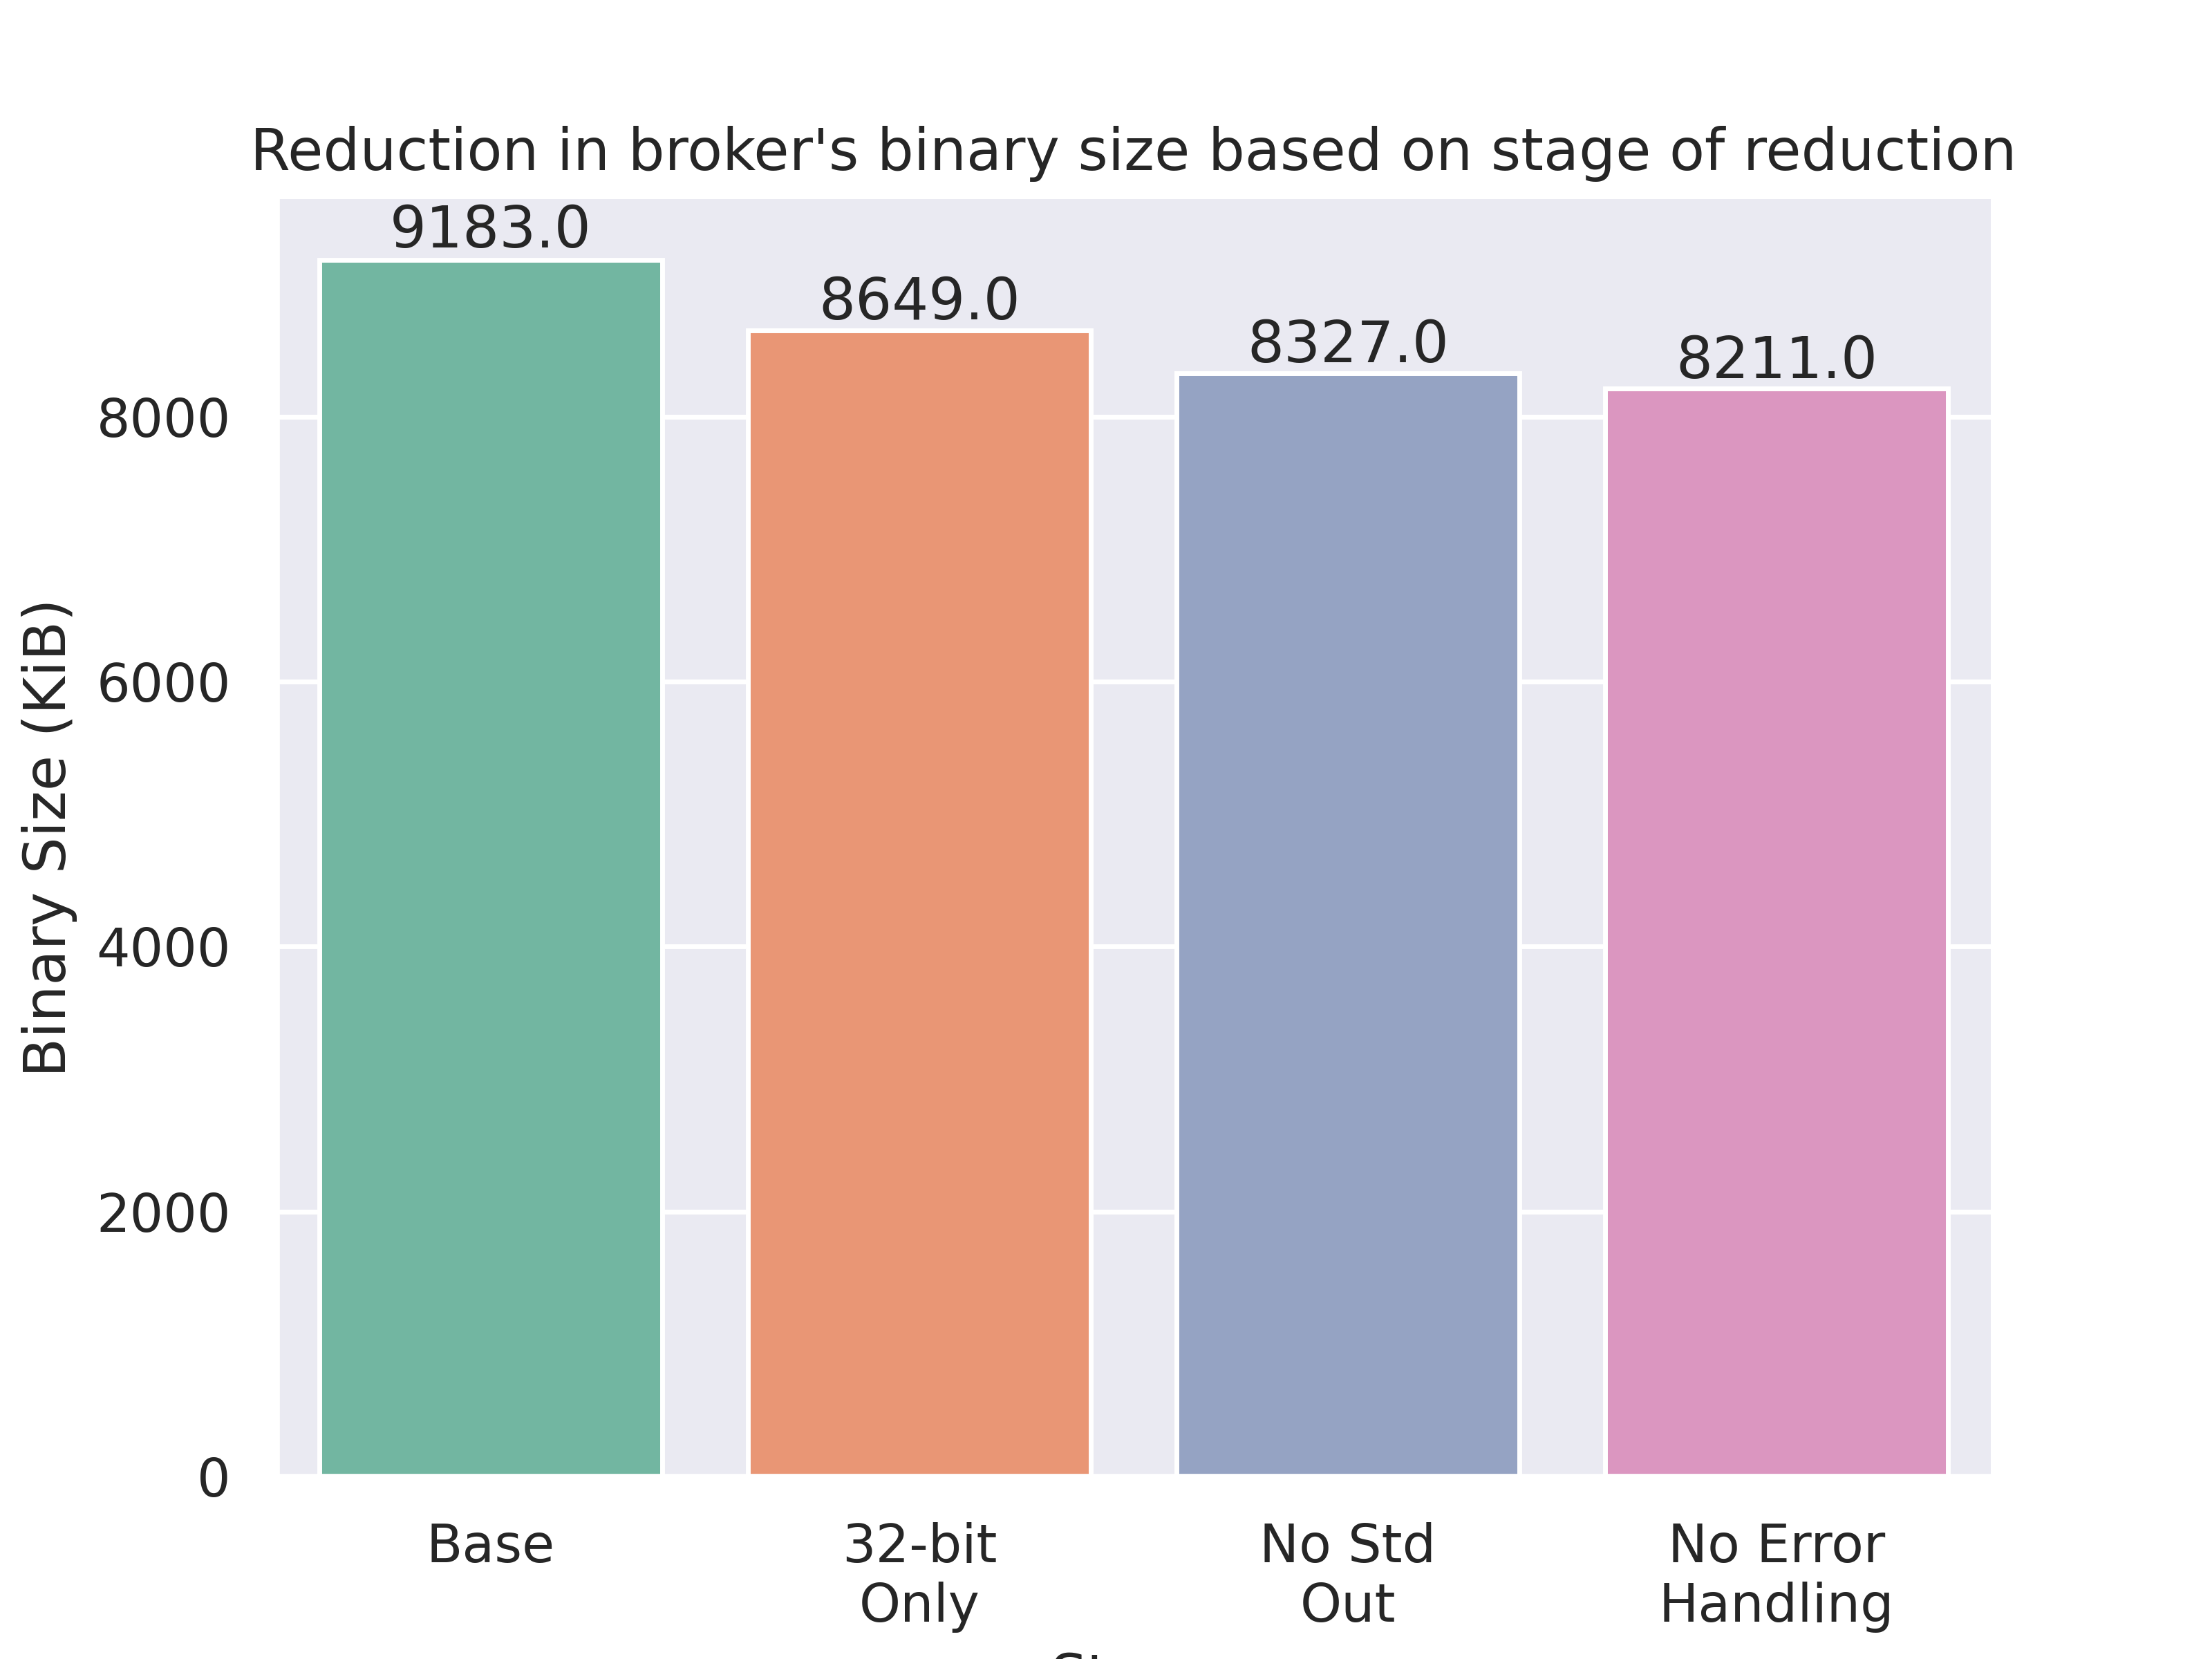
\includegraphics[width=1\linewidth]{images/quinn_binary_reduce_broker.png}
            \caption{Broker binary size reduction.}
            \label{fig:reduce_roker}
        \end{subfigure}
        \caption{The stages of the reduction and the sizes of the QUIC binary at the corresponding stages. Subfigure~\ref{fig:reduce_client} shows the reduction in the binary size of the client and Subfigure~\ref{fig:reduce_roker} shows similar results for the binary size of the broker.
        Compiling in 32-bit only bode results in the highest decrease in binary size.}
        \label{fig:reduce}
    \end{center}
\end{figure}

\subsection{Reducing the QUIC stack}

As we can see from the composition of the binaries of MQuicTT, the QUIC stack is around a third of the size of the implementation.
Hence, we now analyse methods for reducing QUIC's contribution following the previously described methodology.

Figure~\ref{fig:reduce} demonstrates the reduction in binary size at each stage described in the methodology.
Notably, compiling the binary to a 32-bit only target contributes significantly to the reduction of the binary size.
The 32-bit only version of the broker is $5.8\%$ smaller, and the 32-bit only client is $8.5\%$ smaller.
However, the two remaining stages did not contribute significantly to the reduction of the binary sizes.
This can perhaps be attributed to implementation details as the reduction due to error handling and standard output use would be directly proportional to their use in the codebase.
This is further reinforced by the client being reduced by a higher percentage from removing error handling due to the client's source code having more of this feature.

Hence, from the binary analysis conducted, we can see that the QUIC stack contributes a significant amount to the overall binary size of MQuicTT.
We can also see that reducing the size of the QUIC stack is not trivial, with the best results coming from compiling to a 32-bit only target.

Another avenue to reduce the binary size is to look at which features of QUIC and TLS contribute most to the binary size.
We have performed a by feature analysis of the $Quinn$ and $Rustls$ binary contributions using the previously described methodology.

Figure~\ref{fig:mquictt_bin_func} shows the by feature breakdown of the $Quinn$ contribution to the binary size.
Notably, we can see that $Quinn$ heavily leverages a single state machine that handles a lot of logic that may be best abstracted away.
For example, version negotiation does not have its own function and is rather just part of the general connection handling.
Connection migration also does not appear to have its own contribution.

\begin{figure}[t]
    \centering
    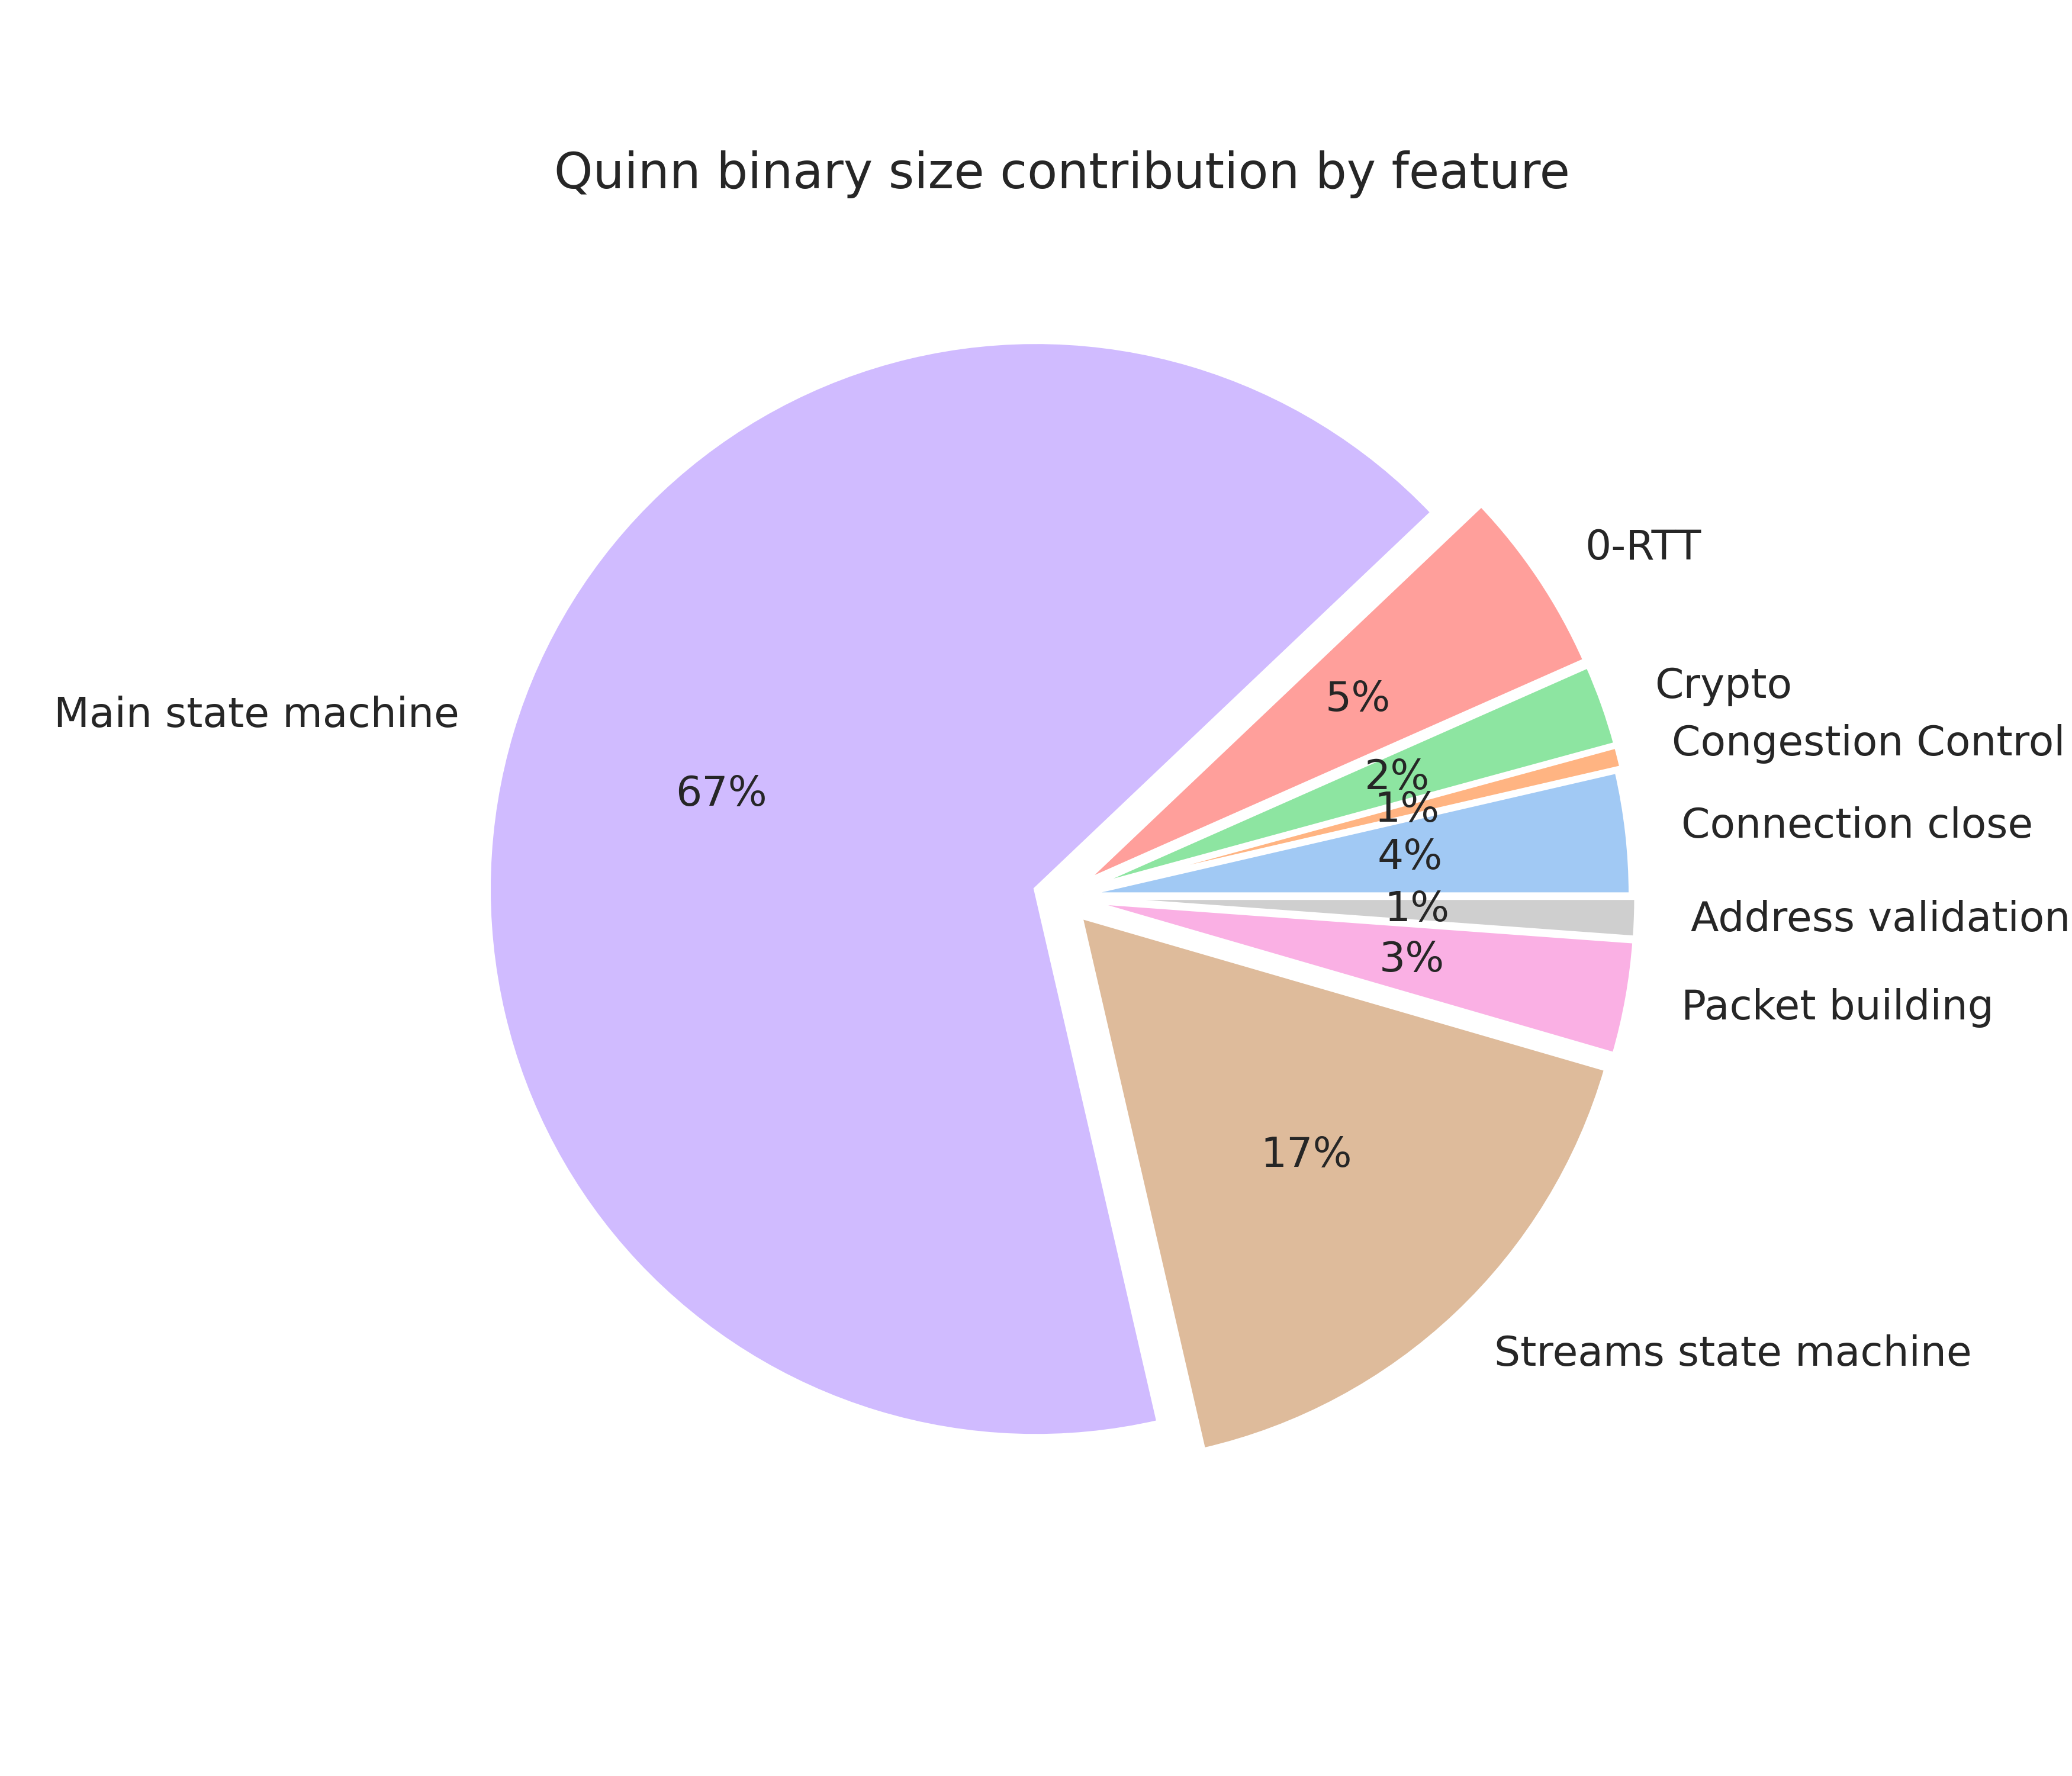
\includegraphics[width=0.75\linewidth]{images/mquictt_binary_by_function.png}
    \caption{A by-feature breakdown of the binary size contribution of $Quinn$ - the QUIC library used for $MQuicTT$. We can see that $Quinn$ heavily leverages the state machine, making the binary size reduction operation quite difficult.}
    \label{fig:mquictt_bin_func}
\end{figure}

As a result, it is difficult to say how much exactly these features contribute to the overall size of the $MQuicTT$ binary.
There are two possible ways to estimate this that we considered.
Firstly, we could look at the number of lines of code and draw some conclusions from this.
However, lines of code do not correspond to binary size well at all; hence, this option was rejected.
Secondly, we could re-write the $Quinn$ implementation with better abstractions, isolating each feature.
However, this is the ideal solution was unfortunately out of scope for this project.

From the features that were extracted successfully, we can see that 0-RTT contributes $5\%$ or $12.2Kb$.
0-RTT connection re-establishment, however, as discussed previously, can be seen as a favourable feature for IoT devices due to its ability to reduce connection time.
In addition to this, removing this feature would not surmount a substantial reduction of $MQuicTT$'s binary size.

Overall, from these results, we can see that the complexity of $QUIC$ in its state machine and handling of streams is the key reason for $Quinn$'s $16\%$ contribution to the size of $MQuicTT$'s binary.

Figure~\ref{fig:tls_bin_func} shows a similar breakdown for $Rustls$.
As expected, the handshake logic contributes most to the size of the binary.
The functions that contribute most to the handshake are the client and server hello handlers.
As QUIC does not use the traditional TLS handshake, it is possible to save space by stripping away the non-QUIC handshake semantics.
It is hard to estimate how much exactly this would remove without making the changes; however, we can approximate this by removing handshake functions that QUIC would definitely not use.
In our approximation, the contribution from the handshake could be reduced from $53\%$ to approximately $44\%$.

\begin{figure}[t]
    \centering
    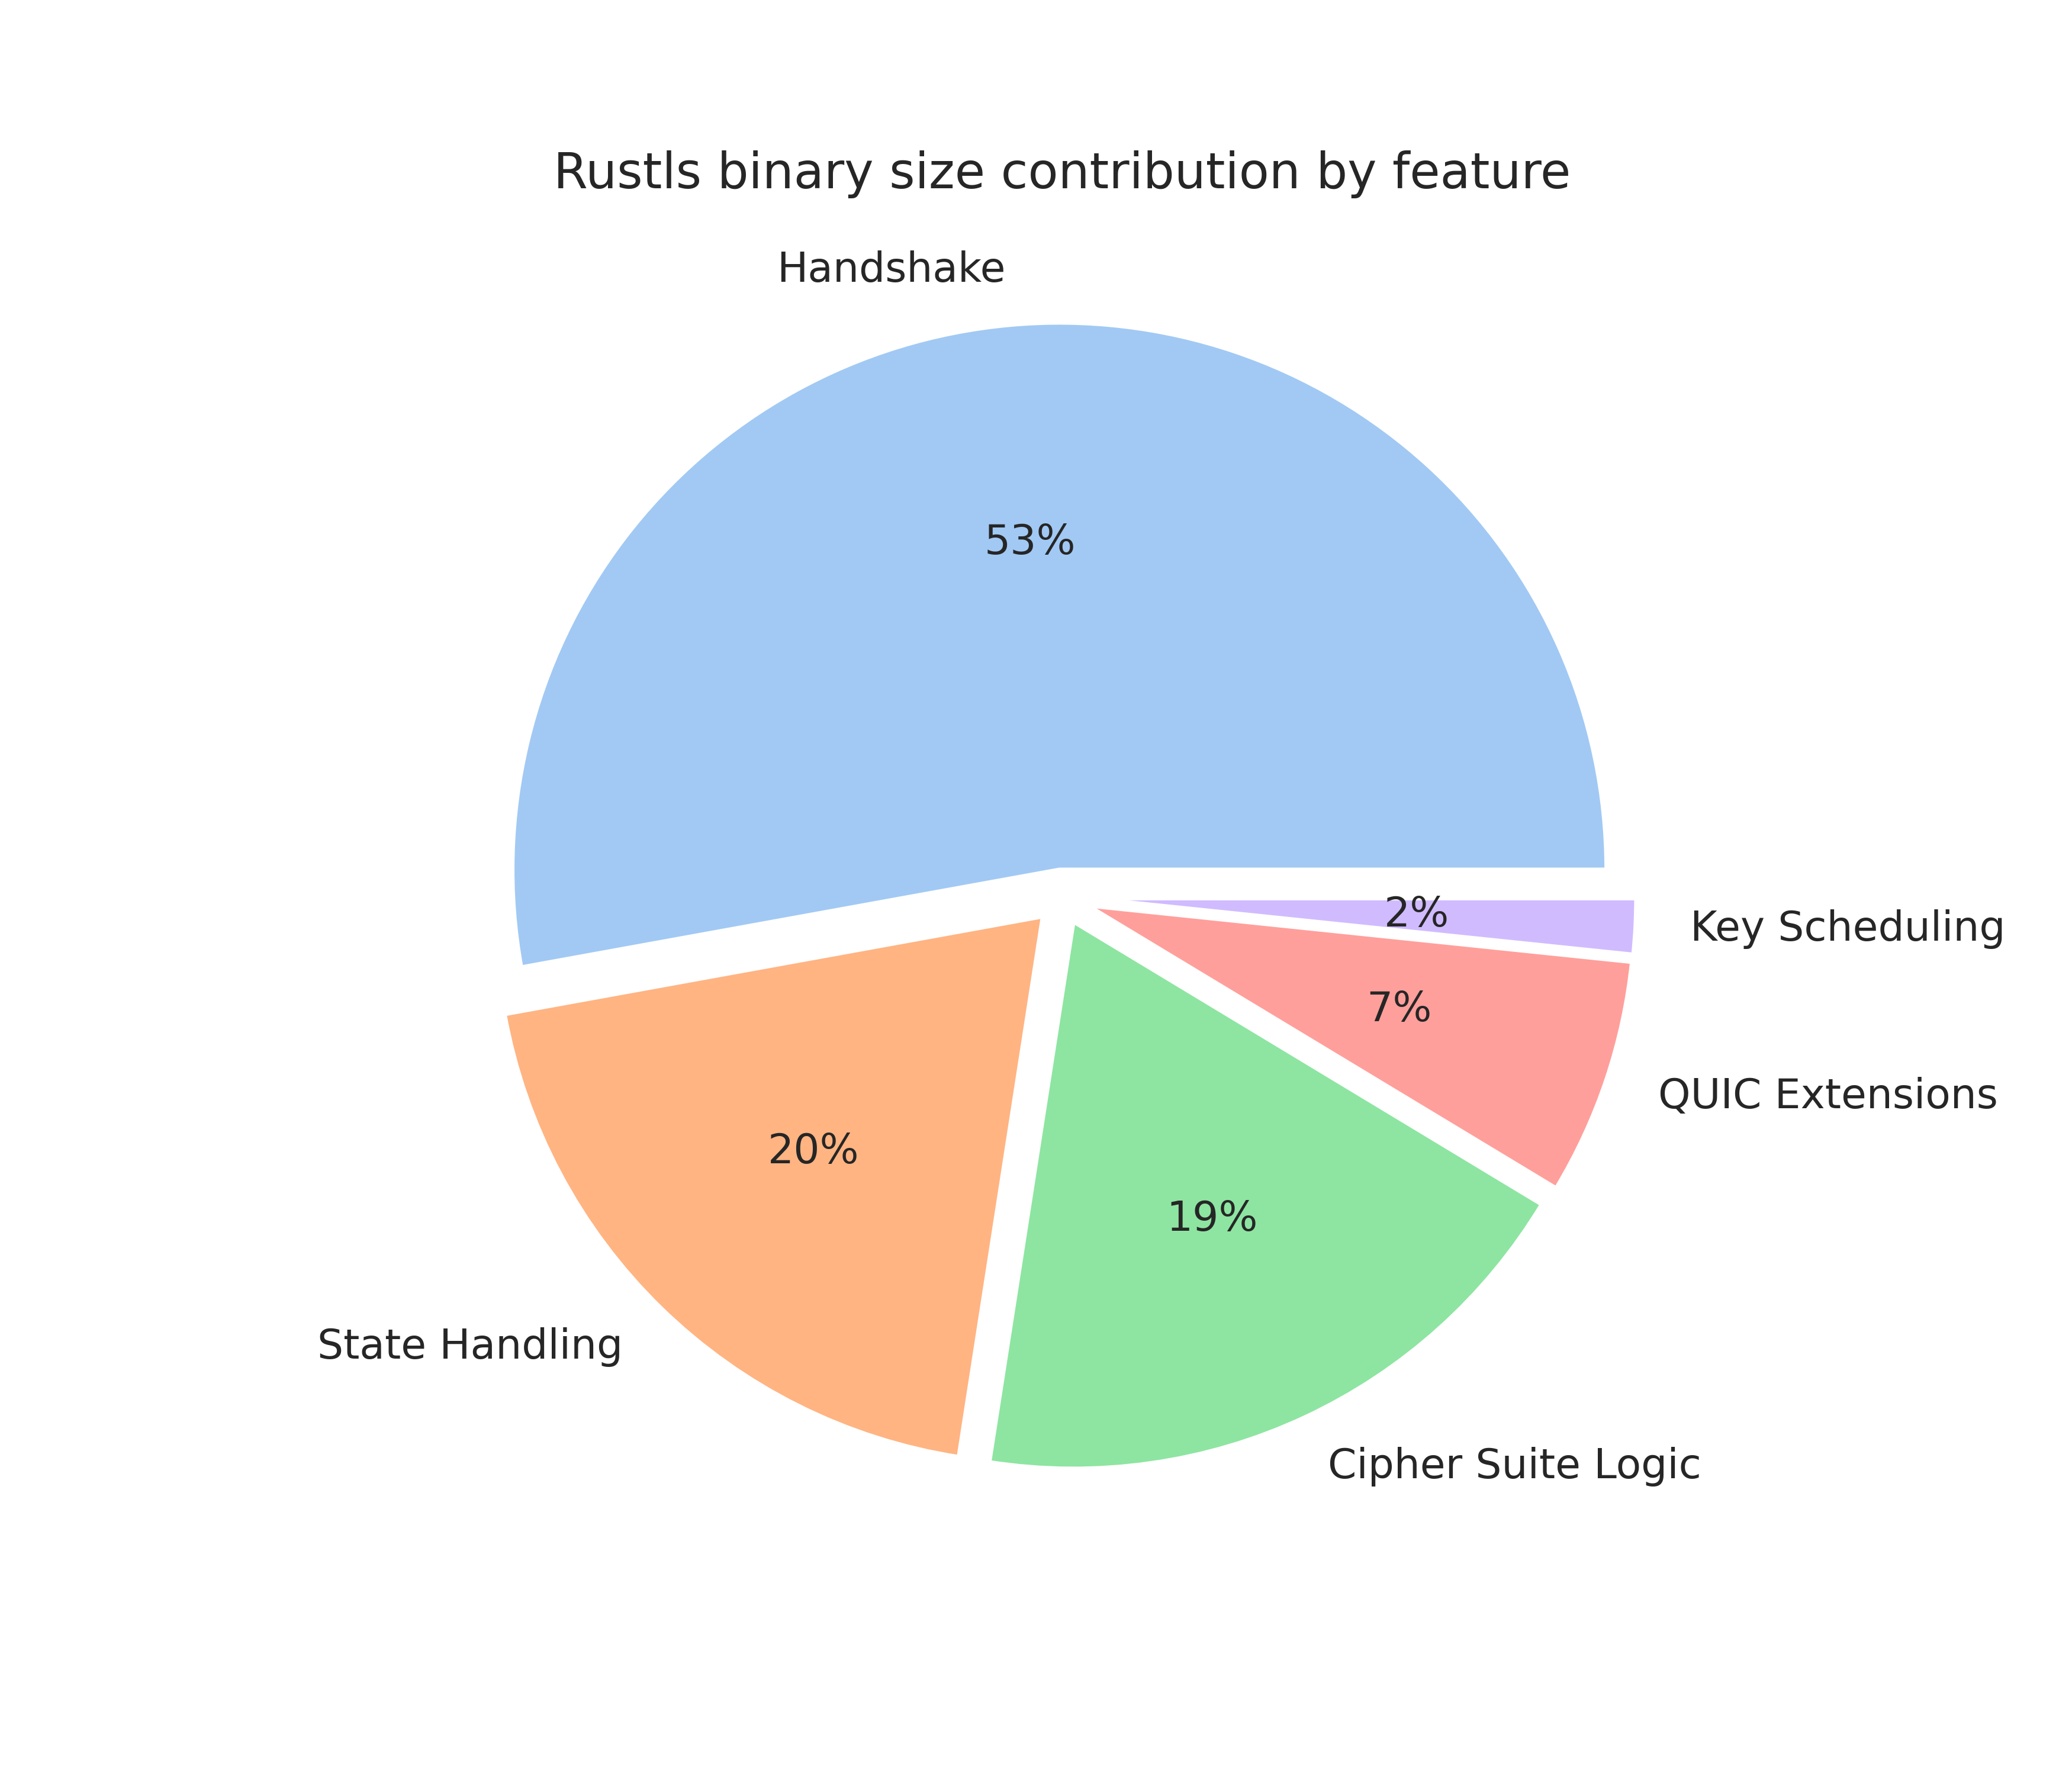
\includegraphics[width=0.75\linewidth]{images/rustls_binary_by_function.png}
    \caption{A by-feature breakdown of the binary size contribution of $Rustls$ - the TLS library used for secure communication. Notably, the new QUIC extensions added to TLS contribute significantly to the binary size contribution.}
    \label{fig:tls_bin_func}
\end{figure}

$Rustls$ also seems to have complex logic for interfacing with and picking cypher suites.
The handling for this is a fifth of $Rustls$'s total binary size contribution.
Some of this logic can perhaps be simplified if the deployment pre-chooses a cypher suite to use.
That is, the library can be changed to interface only with that singular cypher.

Notably, QUIC extensions to $Rustls$ such as in-place encryption and QUIC key generation only contribute $7\%$.
This again shows that if non-QUIC features were to be removed, then we could save on binary size.
However, this is also shows quite a large overhead for applications that do not use QUIC.

In regards to further reductions to the binary size, the contributions made by the standard library include over a thousand functions of approximately the same size.
As we have already removed features such as backtracing, demangling and error reporting, removing these would be risky to the core functionality and would need to be investigated manually.
The most frequently appearing function is $std core::ptr::drop\_in\_place$, which is used by the compiler to execute the destructor of a pointed-to-value.

Overall, the most significant effect to the reduction of the binary size of $MQuicTT$ came from compiling the binary in 32-bit only mode, removing error reporting and handling, and any standard output.
A surprising result is the contribution of the regex library, which can be attributed to the fact that Rust opts to use $utf-8$ instead of $ascii$ for strings.
Reducing the binary size by removing QUIC features may not be the best approach due to limited gains.
However, stripping away non-QUIC features from TLS may reduce the binary size considerably.
